% Construction : M en (0.4, 2.2), centres O₁ en (1.6, 1.2) et O₂ en (3.4, 1.7).
%   M₁ = 2O₁ − M = (2.8, 0.2) ; M₂ = 2O₂ − M₁ = (4, 3.2).
%   Le vecteur MM₂ = (3.6, 1) vaut le double de O₁O₂ = (1.8, 0.5).
% SVG : x = 20 + 44x, y = 160 - 44y.
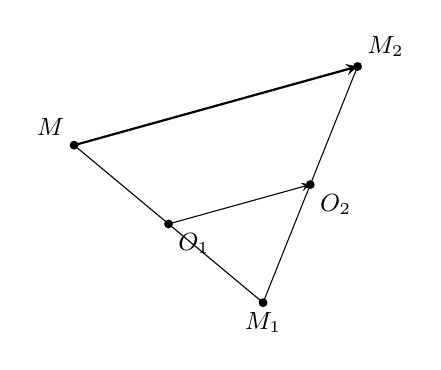
\begin{tikzpicture}[scale=1, >=stealth, every node/.style={font=\small}]
  \draw (0.4, 2.2) -- (2.8, 0.2); \draw (2.8, 0.2) -- (4, 3.2);
  \draw[->, thick] (0.4, 2.2) -- (4, 3.2);
  \draw[->] (1.6, 1.2) -- (3.4, 1.7);
  \foreach \p/\n/\pos in {(0.4, 2.2)/M/above left, (2.8, 0.2)/M_1/below,
                          (4, 3.2)/M_2/above right}
    { \fill \p circle (1.6pt); \node[\pos] at \p {$\n$}; }
  \foreach \p/\n in {(1.6, 1.2)/O_1, (3.4, 1.7)/O_2}
    { \fill \p circle (1.6pt); \node[below right] at \p {$\n$}; }
\end{tikzpicture}
